\input{template.tex}
\usepackage{tkz-euclide}

\begin{document}

\makeheader

Lea recently learned about convex hulls and wanted to
do some more experiments herself.
Therefore, she nailed $n$ nails into a plank of wood and
pulled a rubber band over the nails.
Since Lea nailed nailing the nails, all nails are on
pairwise distinct spots.
But, unfortunately, the rubber band wasn't Convex Hull™ proof!
Instead, it snaps towards its center as illustrated in the figure down below.
\begin{figure}[ht]
  \centering
  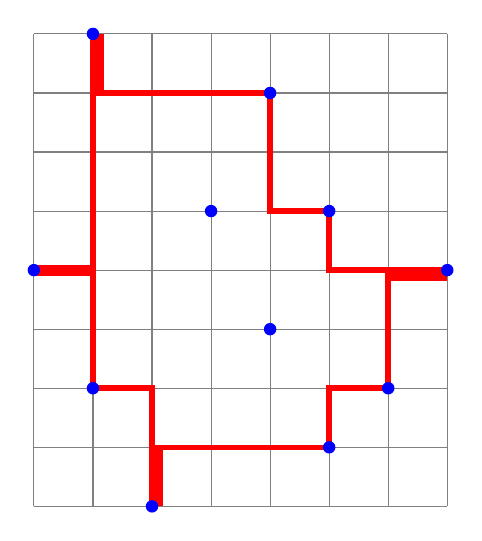
\begin{tikzpicture}[scale=.75]
    \tkzInit[xmax=4,ymax=3,xmin=-3,ymin=-5]
    \tkzGrid
    \tkzAxeXY
    \draw[red, line width=2pt] (2,0) -- (2,-1) -- (4,-1) -- (3,-1)
    -- (3,-3) --(2,-3) -- (2,-4) -- (-1,-4)
    -- (-1,-5) -- (-1,-3) -- (-2,-3) -- (-2,-1)
    -- (-3,-1) -- (-2,-1) -- (-2,3) -- (-2,2)
    -- (1,2) -- (1,0) -- cycle;
    \draw[red, line width=4pt, transform canvas={yshift=-2pt}] (3,-1) -- (4,-1);
    \draw[red, line width=4pt, transform canvas={xshift=2pt}] (-1,-4) -- (-1,-5);
    \draw[red, line width=4pt] (-2,-1) -- (-3,-1);
    \draw[red, line width=4pt, transform canvas={xshift=2pt}] (-2,2) -- (-2,3);
    \foreach \point in {(1,2),(1,-2),(-1,-5),(-2,-3),(-2,3),(4,-1),(3,-3),(2,-4),(2,0),(-3,-1),(0,0)} {
        \fill[blue] \point circle[radius=3pt];
      }
  \end{tikzpicture}
  \caption{Sample \#2. Note: the rubber band sometimes uses some line segments twice (tick lines).}
  \label{fig:convexhull}
\end{figure}
Anyways, Lea still wants to know the length of the rubber band.
Can you help her?

\paragraph*{Input}

The first line contains an integer $n$ ($3 \leq n \leq 2\cdot10^5$) the number of nails.
Then $n$ lines follow, each containing two integers $x_i$ and $y_i$ ($-10^9 \leq x_i, y_i \leq 10^9$)
the coordinates of the $i$-th nail.

\paragraph*{Output}

Print a single integer denoting the length of the rubber band.

\begin{samples}
  \sample{sample1}
  \sample{sample2}
\end{samples}

\end{document}